
\texttt{FastFEM} uses Gmsh\supercite{Gmsh} for mesh generation. Currently, \texttt{v0.0.1} offers two fundamental 2D mesh generation functions, as shown in \autoref{fig:mesh-example1}.  The results of the functions are shown in \autoref{fig:mesh}. \texttt{FastFEM} is fully statically typed so that users can get autocomplete suggestions when writing the function's arguments and using the mesh object it returns.

\pythonCodeBlock{figures/mesher-example1.py}{Two available functions of \texttt{FastFEM v0.0.1} for generating 2D square and rectangle meshes that are shown in \autoref{fig:mesh}.}{fig:mesh-example1}

\begin{figure}[H]
    \centering
    \hfill
    \begin{subfigure}[c]{0.4\textwidth}
        \centering
        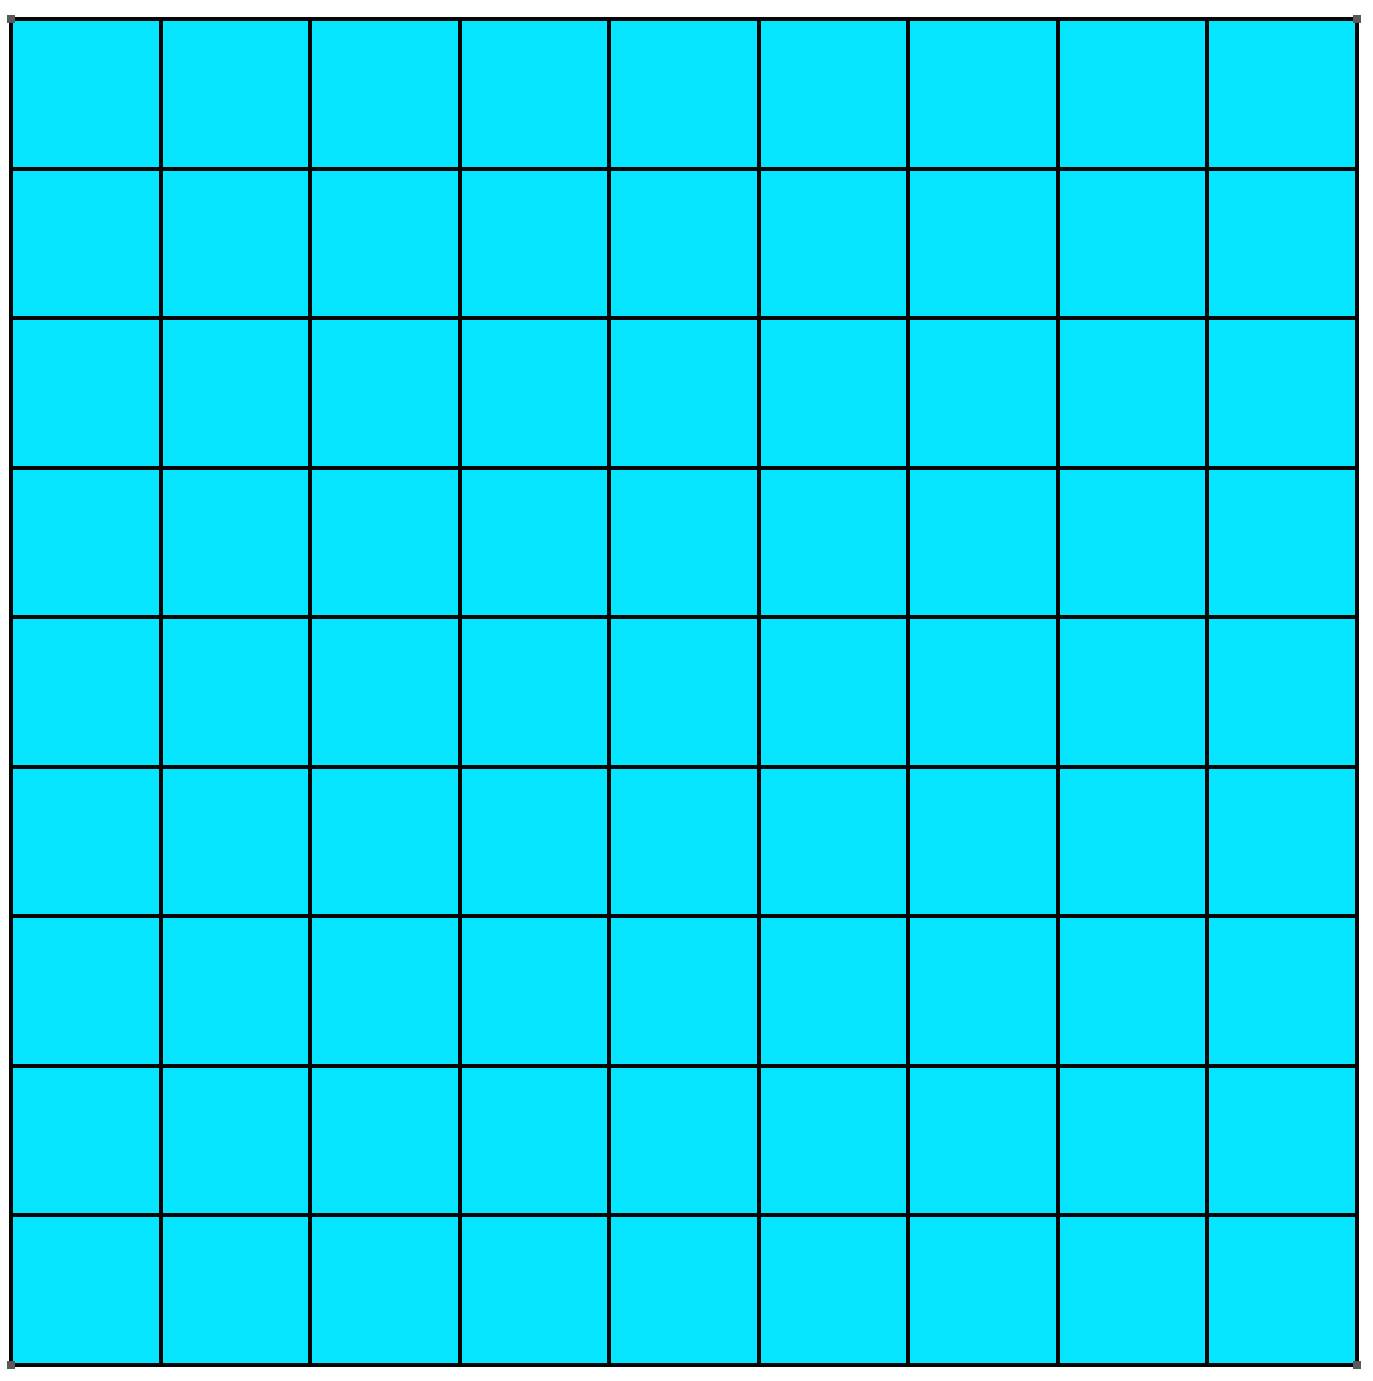
\includegraphics[width=\textwidth]{figures/square_mesh.png}

        \caption{Square mesh.}
        \label{fig:square}
    \end{subfigure}s
    \hspace{0.1\textwidth}
    \begin{subfigure}[c]{0.4\textwidth}
        \centering
        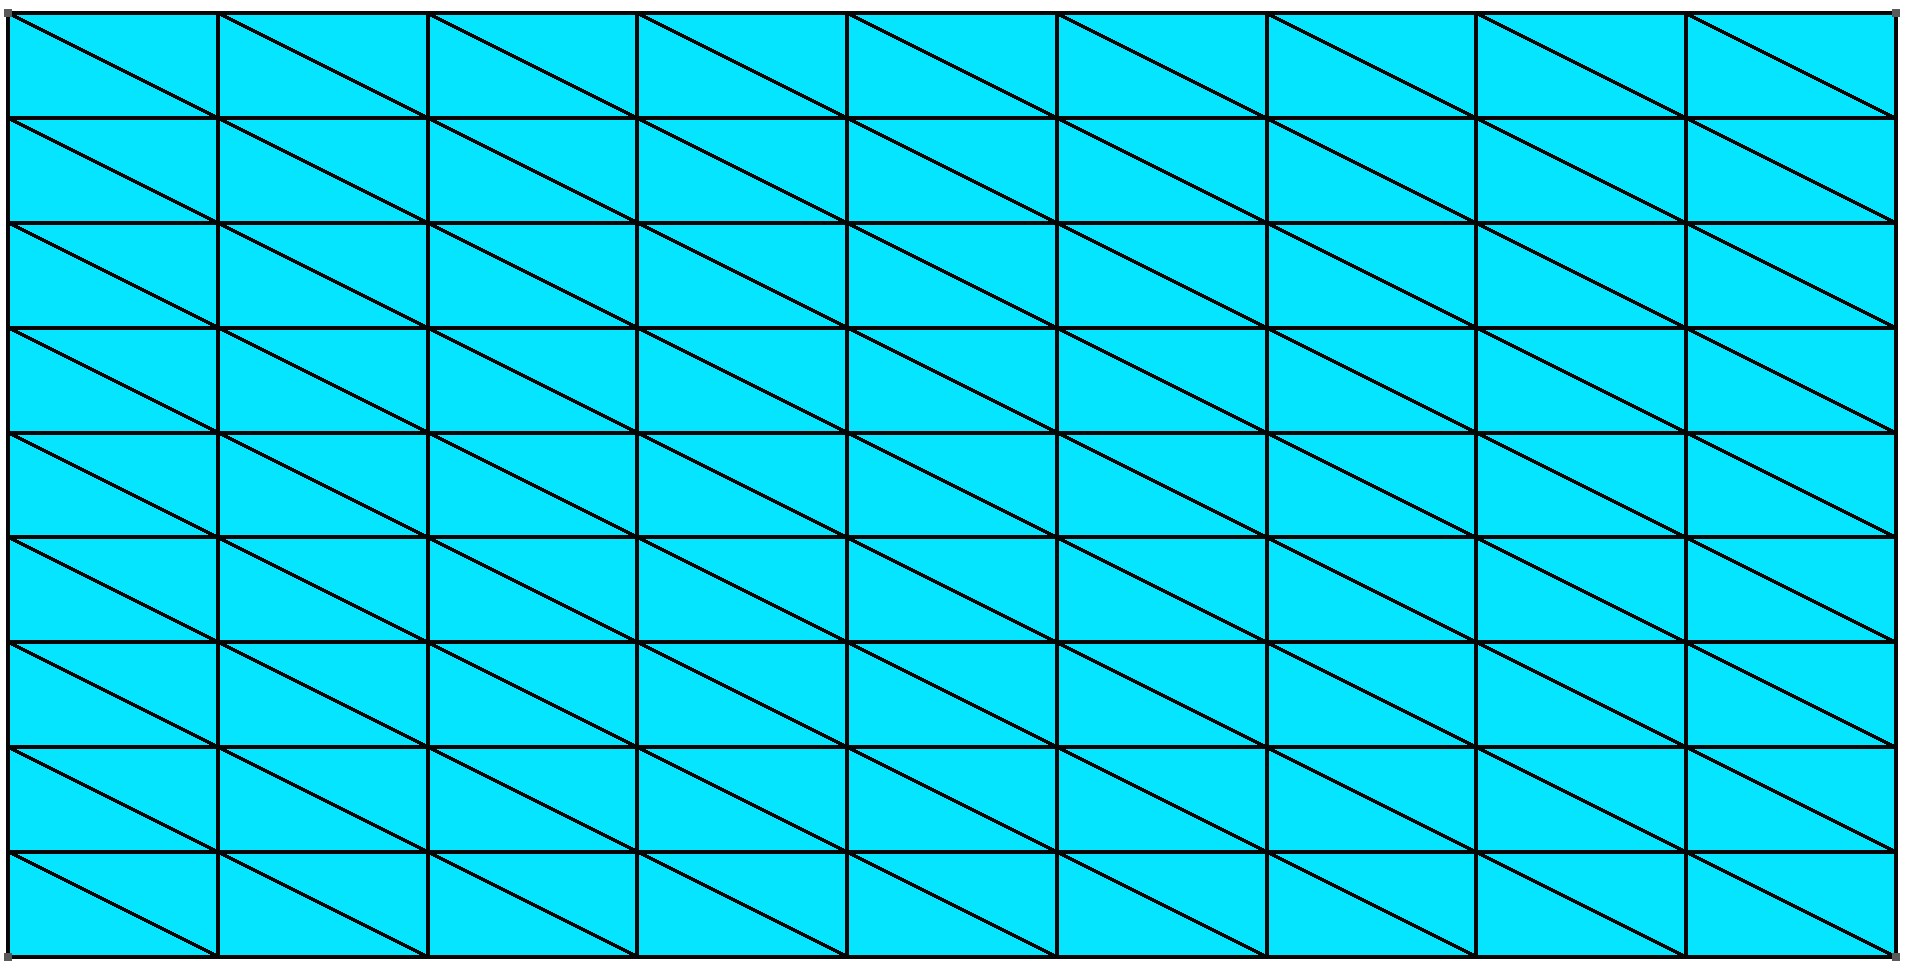
\includegraphics[width=\textwidth]{figures/rectangle_mesh.png}
        \caption{Rectangle mesh.}
        \label{fig:rectangle}
    \end{subfigure}
    \caption{Two examples of mesh generated with the functions in \autoref{fig:mesh-example1}.}
    \label{fig:mesh}
    \hfill
\end{figure}

\texttt{FastFEM v0.0.1} also provides a general-purpose, object-oriented interface for 2D mesh generation by abstracting Gmsh's functional approach. For example, a mesh of an arbitrary 2D geometry, as shown in \autoref{fig:arbitrarymesh}, can be created using the code presented in \autoref{fig:mesh-example2}.

\pythonCodeBlock{figures/mesher-example2.py}{The code that generates the mesh of an arbitrary geometry shown in \autoref{fig:arbitrarymesh}.}{fig:mesh-example2}

\begin{figure}[H]
    \centering
    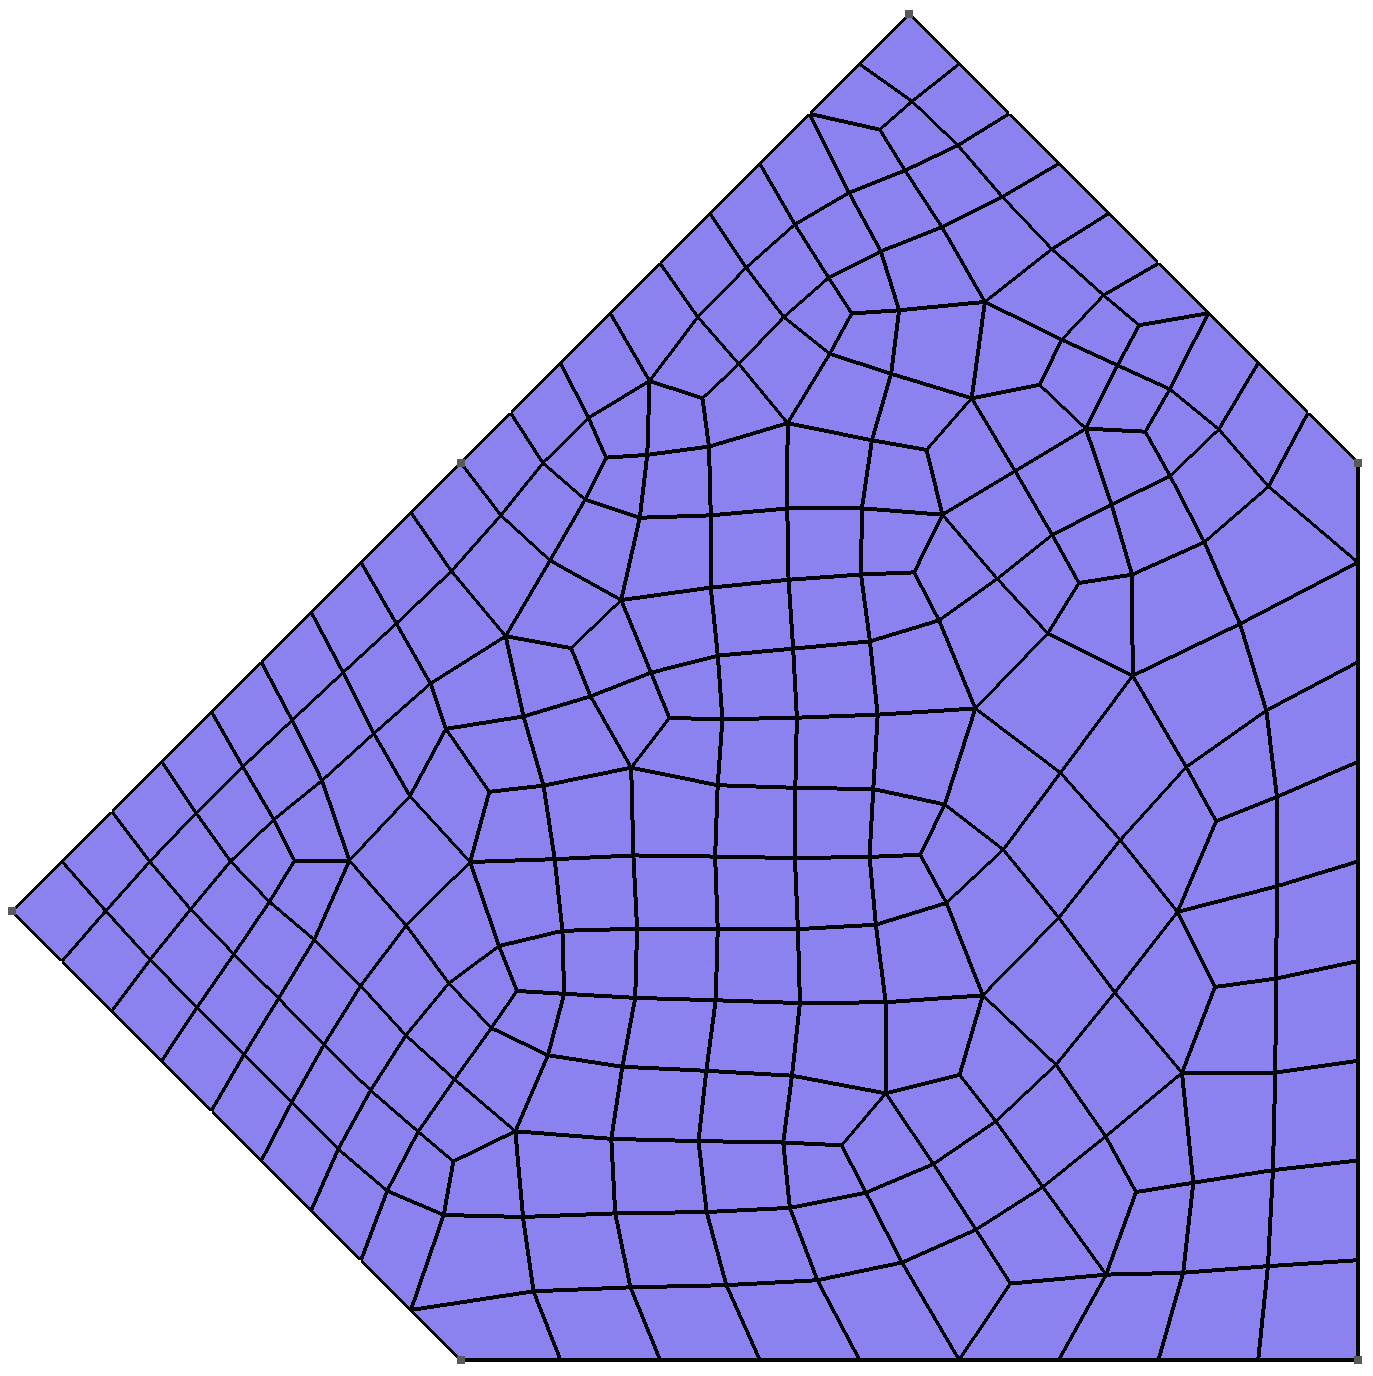
\includegraphics[width=0.5\textwidth]{figures/arbitrary_mesh.png}
    \caption{An arbitrary 2D mesh generated using the code in \autoref{fig:mesh-example2}.}
    \label{fig:arbitrarymesh}
\end{figure}